% Shared preamble of the six stage reports (stages/README.md). Colours and notation are identical in every report.
\documentclass[11pt,a4paper]{article}
\usepackage[margin=2.2cm]{geometry}
\usepackage{amsmath,amssymb,booktabs,graphicx,xcolor,float,caption,subcaption,enumitem,longtable,array}
\usepackage[round]{natbib}
\usepackage[hidelinks]{hyperref}
\usepackage{fancyhdr}
\setlength{\emergencystretch}{2em}
\setlength{\parskip}{3pt}
\definecolor{roigreen}{RGB}{0,160,0}
\definecolor{artred}{RGB}{220,0,0}
\definecolor{maskblue}{RGB}{31,119,180}
\definecolor{ermgrey}{RGB}{110,110,110}
\definecolor{supported}{RGB}{0,120,0}
\definecolor{notsupported}{RGB}{190,0,0}
\newcommand{\ok}{\textcolor{supported}{\textbf{supported}}}
\newcommand{\no}{\textcolor{notsupported}{\textbf{not supported}}}
\newcommand{\mixed}{\textcolor{orange!80!black}{\textbf{partly supported}}}
\newcommand{\roi}{\textcolor{roigreen}{ROI}}
\newcommand{\na}{\textit{n/a}}
\newcommand{\registered}[1]{\textsf{registered before results (#1)}}
\newcommand{\posthoc}[1]{\textsf{post hoc (#1)}}
\pagestyle{fancy}\fancyhf{}\rhead{\small Where the Shortcut Sits --- stage reports}\lfoot{\small\leftmark}\rfoot{\small\thepage}
\newcommand{\stagebox}[1]{\noindent\colorbox{gray!12}{\parbox{\dimexpr\linewidth-2\fboxsep}{\small #1}}\par\medskip}

% generated by make_stage*.py from result files; do not edit
\providecommand{\sThreeNAisic}{3597}
\providecommand{\sThreeNBisic}{5381}
\providecommand{\sThreeNZeroisic}{863}
\providecommand{\sThreeNAthyroid}{1150}
\providecommand{\sThreeNBthyroid}{326}
\providecommand{\sThreeNZerothyroid}{1801}
\providecommand{\sThreeNAovary}{617}
\providecommand{\sThreeNBovary}{194}
\providecommand{\sThreeNZeroovary}{348}
\providecommand{\sThreeNAcapsule}{816}
\providecommand{\sThreeNBcapsule}{1240}
\providecommand{\sThreeNZerocapsule}{507}
\providecommand{\sThreeAisicDINOvTwo}{$-0.049$ [$-0.083, -0.018$]}
\providecommand{\sThreeBisicDINOvTwo}{$+0.098$ [$+0.060, +0.136$]}
\providecommand{\sThreeXisicDINOvTwo}{$+0.147$ [$+0.111, +0.185$]}
\providecommand{\sThreeErmAisicDINOvTwo}{0.510}
\providecommand{\sThreeErmBisicDINOvTwo}{0.510}
\providecommand{\sThreeMaskCorrAisicDINOvTwo}{0.917}
\providecommand{\sThreeMaskRevAisicDINOvTwo}{0.460}
\providecommand{\sThreeAisicDermLIP}{$-0.104$ [$-0.143, -0.067$]}
\providecommand{\sThreeBisicDermLIP}{$-0.090$ [$-0.135, -0.046$]}
\providecommand{\sThreeXisicDermLIP}{$+0.014$ [$-0.037, +0.063$]}
\providecommand{\sThreeErmAisicDermLIP}{0.665}
\providecommand{\sThreeErmBisicDermLIP}{0.735}
\providecommand{\sThreeMaskCorrAisicDermLIP}{0.884}
\providecommand{\sThreeMaskRevAisicDermLIP}{0.561}
\providecommand{\sThreeAthyroidDINOvTwo}{$+0.109$ [$+0.085, +0.133$]}
\providecommand{\sThreeBthyroidDINOvTwo}{$+0.348$ [$+0.307, +0.388$]}
\providecommand{\sThreeXthyroidDINOvTwo}{$+0.239$ [$+0.196, +0.280$]}
\providecommand{\sThreeErmAthyroidDINOvTwo}{0.289}
\providecommand{\sThreeErmBthyroidDINOvTwo}{0.405}
\providecommand{\sThreeMaskCorrAthyroidDINOvTwo}{0.908}
\providecommand{\sThreeMaskRevAthyroidDINOvTwo}{0.398}
\providecommand{\sThreeAthyroidMedSigLIP}{$+0.053$ [$+0.032, +0.073$]}
\providecommand{\sThreeBthyroidMedSigLIP}{$+0.248$ [$+0.200, +0.293$]}
\providecommand{\sThreeXthyroidMedSigLIP}{$+0.195$ [$+0.153, +0.238$]}
\providecommand{\sThreeErmAthyroidMedSigLIP}{0.289}
\providecommand{\sThreeErmBthyroidMedSigLIP}{0.481}
\providecommand{\sThreeMaskCorrAthyroidMedSigLIP}{0.912}
\providecommand{\sThreeMaskRevAthyroidMedSigLIP}{0.341}
\providecommand{\sThreeAovaryDINOvTwo}{$+0.132$ [$+0.072, +0.196$]}
\providecommand{\sThreeBovaryDINOvTwo}{$+0.302$ [$+0.225, +0.378$]}
\providecommand{\sThreeXovaryDINOvTwo}{$+0.170$ [$+0.087, +0.252$]}
\providecommand{\sThreeErmAovaryDINOvTwo}{0.413}
\providecommand{\sThreeErmBovaryDINOvTwo}{0.423}
\providecommand{\sThreeMaskCorrAovaryDINOvTwo}{0.828}
\providecommand{\sThreeMaskRevAovaryDINOvTwo}{0.545}
\providecommand{\sThreeAcapsuleDINOvTwo}{$+0.084$ [$+0.055, +0.112$]}
\providecommand{\sThreeBcapsuleDINOvTwo}{$+0.461$ [$+0.415, +0.506$]}
\providecommand{\sThreeXcapsuleDINOvTwo}{$+0.377$ [$+0.327, +0.426$]}
\providecommand{\sThreeErmAcapsuleDINOvTwo}{0.581}
\providecommand{\sThreeErmBcapsuleDINOvTwo}{0.429}
\providecommand{\sThreeMaskCorrAcapsuleDINOvTwo}{0.972}
\providecommand{\sThreeMaskRevAcapsuleDINOvTwo}{0.665}
\providecommand{\sThreeAcapsuleMedSigLIP}{$+0.117$ [$+0.088, +0.147$]}
\providecommand{\sThreeBcapsuleMedSigLIP}{$+0.452$ [$+0.407, +0.495$]}
\providecommand{\sThreeXcapsuleMedSigLIP}{$+0.335$ [$+0.286, +0.383$]}
\providecommand{\sThreeErmAcapsuleMedSigLIP}{0.570}
\providecommand{\sThreeErmBcapsuleMedSigLIP}{0.464}
\providecommand{\sThreeMaskCorrAcapsuleMedSigLIP}{0.977}
\providecommand{\sThreeMaskRevAcapsuleMedSigLIP}{0.687}
\providecommand{\sThreeNRuns}{7}
\providecommand{\sThreeNXPos}{6}
\providecommand{\sThreeSrcHAM}{$-0.011$ [$-0.064, +0.043$]}
\providecommand{\sThreeSrcBCN}{$-0.067$ [$-0.110, -0.025$]}
\providecommand{\sThreeHairRatioMedian}{0.033}
\providecommand{\sThreeEOneTwomask}{$-0.103$ [$-0.121, -0.085$]}
\providecommand{\sThreeEOneTwobalanced}{$+0.160$ [$+0.144, +0.177$]}
\providecommand{\sThreeEOneTwodfr}{$+0.179$ [$+0.148, +0.211$]}
\providecommand{\sThreeUnetDice}{0.886}
\providecommand{\sThreeUnetHam}{0.895}
\providecommand{\sThreeHairDetIoU}{0.222}
\providecommand{\sThreeProbeIoU}{0.625}
\providecommand{\sThreeProbeAcc}{0.922}
\providecommand{\sThreeNPrimary}{16}
\providecommand{\sThreeNPrimaryOK}{11}
\providecommand{\sThreeNPOneOK}{4}
\providecommand{\sThreePPOneISIC}{$+0.147$ [$+0.111, +0.185$]}
\providecommand{\sThreePHolmPOneISIC}{0.0016}
\providecommand{\sThreePPOneThyroid}{$+0.239$ [$+0.196, +0.280$]}
\providecommand{\sThreePHolmPOneThyroid}{0.0016}
\providecommand{\sThreePPOneCapsule}{$+0.377$ [$+0.327, +0.426$]}
\providecommand{\sThreePHolmPOneCapsule}{0.0016}
\providecommand{\sThreePPOneOvary}{$+0.170$ [$+0.087, +0.252$]}
\providecommand{\sThreePHolmPOneOvary}{0.0016}
\providecommand{\sThreePPTwoISIC}{$+0.042$ [$+0.024, +0.058$]}
\providecommand{\sThreePHolmPTwoISIC}{0.0016}
\providecommand{\sThreePPTwoThyroid}{$+0.283$ [$+0.237, +0.329$]}
\providecommand{\sThreePHolmPTwoThyroid}{0.0016}
\providecommand{\sThreePPTwoCapsule}{$-0.006$ [$-0.018, +0.006$]}
\providecommand{\sThreePHolmPTwoCapsule}{0.3486}
\providecommand{\sThreePPTwoOvary}{$+0.043$ [$+0.023, +0.065$]}
\providecommand{\sThreePHolmPTwoOvary}{0.0016}
\providecommand{\sThreePPThreeISIC}{$+0.035$ [$+0.017, +0.055$]}
\providecommand{\sThreePHolmPThreeISIC}{0.0016}
\providecommand{\sThreePPThreeThyroid}{$+0.215$ [$+0.189, +0.244$]}
\providecommand{\sThreePHolmPThreeThyroid}{0.0016}
\providecommand{\sThreePPThreeCapsule}{$-0.139$ [$-0.158, -0.120$]}
\providecommand{\sThreePHolmPThreeCapsule}{0.0016}
\providecommand{\sThreePPThreeOvary}{$+0.035$ [$+0.003, +0.067$]}
\providecommand{\sThreePHolmPThreeOvary}{0.1304}
\providecommand{\sThreePPFourISIC}{$-0.028$ [$-0.064, +0.007$]}
\providecommand{\sThreePHolmPFourISIC}{0.3486}
\providecommand{\sThreePPFourThyroid}{$+0.110$ [$+0.079, +0.142$]}
\providecommand{\sThreePHolmPFourThyroid}{0.0016}
\providecommand{\sThreePPFourCapsule}{$+0.079$ [$+0.042, +0.115$]}
\providecommand{\sThreePHolmPFourCapsule}{0.0016}
\providecommand{\sThreePPFourOvary}{$+0.031$ [$-0.014, +0.077$]}
\providecommand{\sThreePHolmPFourOvary}{0.3486}
\providecommand{\sThreeNCxr}{4}
\providecommand{\sThreeRegIsic}{\texttt{76e25d4}, 2026-09-26 13:14}
\providecommand{\sThreeRegThy}{\texttt{ea57661}, 2026-09-26 22:46}
\providecommand{\sThreeRegOv}{\texttt{2517600}, 2026-09-27 07:29}
\providecommand{\sThreeRegCap}{\texttt{fcbf8d9}, 2026-09-27 00:40}
\providecommand{\sThreeRegCxr}{\texttt{4d1a924}, 2026-09-26 18:07}
\providecommand{\sThreeRegStat}{\texttt{4e9d44c}, 2026-09-27 09:37}
\providecommand{\sThreeRegRep}{\texttt{2699d51}, 2026-09-26 15:47}
\providecommand{\sThreeRegFinal}{\texttt{c45d482}, 2026-09-28 00:35}
\providecommand{\sThreeExRisichairinroi}{0.534}
\providecommand{\sThreeExRisichairoutroi}{0.000}
\providecommand{\sThreeExRovarycalipersinroi}{1.000}
\providecommand{\sThreeExRovarycalipersoutroi}{0.000}
\providecommand{\sThreeExRcapsuledebrisinroi}{0.740}
\providecommand{\sThreeExRcapsuledebrisoutroi}{0.005}

\title{\textbf{Stage 3 --- Real artifacts across modalities}\\[3pt]\large Where the Shortcut Sits: supervisor meeting 3 of 6}
\author{}
\date{Report generated from the repository on \today}
\begin{document}
\maketitle
\stagebox{\textbf{In one sentence.} With real, unedited artifacts --- hair in dermoscopy, calipers in thyroid and
ovarian ultrasound, debris in capsule endoscopy --- ROI masking helps far more when the artifact lies outside the ROI
than when it lies inside it (crossover positive in \sThreeNXPos{} of \sThreeNRuns{} cohort--encoder pairs and in all
four pre-specified primary tests after Holm correction); the dermatology encoder DermLIP and real chest-radiograph
devices are the exceptions.}
% Shared notation. Each stage defines \notY, \notA, \notROI, \notCross, \notCI and \notExtra before \input-ing this
% file, so that a report only names the cohorts and quantities it has already introduced.
\section*{Notation}
\begin{tabular}{p{3.2cm}p{11.8cm}}
$Y\in\{0,1\}$ & diagnosis: \notY. \\
$A\in\{0,1\}$ & artifact present: \notA. \\
ROI & region of interest: \notROI; drawn in \textcolor{roigreen}{green}; artifacts in \textcolor{artred}{red}. \\
$r$ & overlap $|\text{artifact}\cap\text{ROI}|/|\text{artifact}|$. Trap~A: $r\ge0.5$ (artifact in the ROI); Trap~B: $r<0.1$ (outside). \\
Environments & training and correlated test $P(A{=}1\mid Y{=}1)=0.9$, $P(A{=}1\mid Y{=}0)=0.1$; reversed test 0.1/0.9; clean test: artifact independent of $Y$ (real artifacts: half of each class) or absent (synthetic artifacts). \\
ERM, mask & linear head on the frozen features of the original image / of the ROI-masked image. \\
Crossover & \notCross \\
CI & \notCI \\
$|\Delta p|$ & same-head counterfactual sensitivity: change of the predicted probability when the artifact is inserted into the same image. \\
\notExtra
\end{tabular}


\section{Where we are}
Stage~2 established the location law with synthetic artifacts whose position was controlled. Synthetic artifacts
answer \emph{whether} location can matter; they cannot show that it matters for the artifacts clinicians actually
produce. This meeting moves to real artifacts, whose location is read from masks rather than set by us. It also
reports a design that failed (the E12 overlap contrast), how well the automatic artifact masks agree with the images,
where the law does not hold (chest radiography), and the pre-specified 16-test confirmatory family. All intervals are
from regenerated runs with the corrected bootstrap; the chest-radiograph device runs could not be regenerated and are
shown as point estimates only.

\section{Question}
\begin{enumerate}[label=\textbf{Q3\alph*},leftmargin=*]\itemsep1pt
\item With real artifacts and the same protocol, is ROI masking less useful --- or harmful --- when the artifact lies
inside the ROI than when it lies outside it (a positive \emph{crossover})?
\item Does this hold across modalities, artifacts and encoders?
\item Are the artifact masks that define ``inside'' and ``outside'' good enough to support the answer?
\end{enumerate}
\paragraph{Design: two traps sharing one artifact-free group} A real artifact's location is fixed by the image, so we
cannot move it. Instead each cohort is split into images whose artifact lies mostly inside the ROI (overlap $r\ge0.5$,
\emph{Trap~A}) and images whose artifact lies outside it ($r<0.1$, \emph{Trap~B}). Each trap is completed by the same
artifact-free images and receives the trap environments of Stage~1 (training and correlated test 0.9/0.1, reversed
test 0.1/0.9). The primary quantity is the \emph{crossover}
$\big[\mathrm{mask}-\mathrm{ERM}\big]_{B}-\big[\mathrm{mask}-\mathrm{ERM}\big]_{A}$ on the reversed test: the law
predicts it is positive.
\paragraph{Rejected: the overlap-contrast design (E12)} The pilot compared inside-ROI with outside-ROI artifacts
directly, without an artifact-free group. That design makes ``artifact inside'' versus ``artifact outside'' the label
proxy; masking then removes exactly the outside artifacts that define one side of the contrast and keeps the inside
ones that define the other, so masking is expected to harm by construction and the result says nothing about
location. Section~\ref{sec:e12} shows it.

\section{Methods}
\paragraph{Cohorts} Table~\ref{tab:cohorts}. Dermoscopy: ISIC 2019 \citep{combalia2019bcn,tschandl2018ham} with the
published semi-automatic hair masks \citep{wegley2026artifacts}; lesion masks are HAM10000 manual masks or, for BCN and
MSK images, a U-Net trained on ISIC 2018 Task~1 only \citep{codella2019isic}. Thyroid: TN3K images
\citep{gong2021tn3k} with the TNCD malignancy labels and nodule masks; calipers segmented by a rule-based detector.
Ovary: MMOTU \citep{zhao2022mmotu} tumour masks and a caliper detector. Capsule endoscopy: SEE-AI \citep{seeai2023}
expert lesion boxes and debris masks from a patch-token probe trained on expert-masked frames.
\paragraph{Protocol (E13)} Frozen encoders (DINOv2 ViT-B/14 @518 for every cohort; DermLIP for dermoscopy, MedSigLIP-448
for thyroid and capsule), logistic heads, 5 seeds $\times$ 5 grouped folds (groups: lesion identifier and perceptual
hash; capsule: blocks of 100 frame numbers plus hash duplicates, since no video identifiers are published). Within
each label the artifact-bearing images are subsampled to the source mix of the artifact-free group (source matching).
\paragraph{Statistics} Crossed seed $\times$ image bootstrap, 10,000 replicates; the crossover's interval resamples
the same images in both traps. The 16-test primary family is Holm-corrected; everything else is reported with
unadjusted 95\% intervals.

\section{Experiments}
\begin{table}[H]\centering\scriptsize
\caption{Experiments of this stage with registration status, the registration document (\texttt{docs/PREREGISTRATION\_<name>.md}), its first commit and the support criterion stated in advance. Commit times are set by the committing machine and are not independent proof of order.}\label{tab:exp}
\begin{tabular}{p{3.1cm}p{2.1cm}p{2.4cm}p{3.2cm}p{3.3cm}}\toprule
Experiment & Status & Registration & First commit (local time) & Support criterion \\\midrule
Dermoscopy hair traps (E13, DINOv2) & \ok{} registered & ISIC2019\_\allowbreak{}TRAPS & \texttt{76e25d4}, 2026-09-26 13:14 & crossover CI $>0$ \\
Dermoscopy hair, DermLIP & \ok{} registered & ISIC2019\_\allowbreak{}TRAPS & \texttt{76e25d4}, 2026-09-26 13:14 & crossover CI $>0$ \\
Thyroid caliper traps & \ok{} registered & THYROID\_\allowbreak{}TRAPS & \texttt{ea57661}, 2026-09-26 22:46 & crossover CI $>0$ \\
Ovarian caliper traps & \ok{} registered & OVARY\_\allowbreak{}TRAPS & \texttt{2517600}, 2026-09-27 07:29 & crossover CI $>0$ \\
Capsule debris traps & \ok{} registered & CAPSULE\_\allowbreak{}TRAPS & \texttt{fcbf8d9}, 2026-09-27 00:40 & crossover CI $>0$ \\
Chest-radiograph device traps & \ok{} registered & CXR\_\allowbreak{}DEVICE\_\allowbreak{}TRAPS & \texttt{4d1a924}, 2026-09-26 18:07 & crossover CI $>0$ \\
Location tests P1 (four cohorts, Holm) & \mixed{} each test registered; Holm grouping post hoc & STATISTICAL\_\allowbreak{}PLAN & \texttt{4e9d44c}, 2026-09-27 09:37 & Holm $p<0.05$, positive estimate \\
Chest drains (NIH) & \ok{} registered & CXR\_\allowbreak{}DRAIN & \texttt{3d0cffc}, 2026-09-27 03:29 & mask $-$ ERM reported with CI, no direction \\
Crossed-bootstrap intervals (A1) & \ok{} registered & FINAL (A1) & \texttt{c45d482}, 2026-09-28 00:35 & a claim is stated only if its crossed CI excludes 0 \\
\bottomrule\end{tabular}
\end{table}

\textbf{Caveat on the primary family.} The 16 tests were grouped into one Holm family after the individual results
were known (the statistical plan \sThreeRegStat{} was written after the first trap results). Each test was registered
with its cohort; the grouping is therefore conservative bookkeeping, not a pre-registered family.

\section{Results}
\subsection{Cohorts and masks}
\begin{table}[H]\centering\scriptsize
\caption{Real-artifact cohorts and pool sizes (images, positive/negative diagnosis) before the environments are sampled. Trap A: artifact mostly inside the ROI ($r\ge0.5$); Trap B: outside ($r<0.1$); both share the artifact-free group.}\label{tab:cohorts}
\resizebox{\linewidth}{!}{\begin{tabular}{p{3.4cm}p{2.4cm}p{2.5cm}p{2.2cm}ccc}\toprule
Cohort & Task & Artifact (mask source) & ROI & Artifact-free pos/neg & Trap A pos/neg & Trap B pos/neg \\\midrule
ISIC 2019 dermoscopy (HAM10000, BCN20000, MSK) & melanoma vs other & hair (published masks) & lesion: HAM manual / U-Net & 157/706 & 942/2655 & 969/4412 \\
TN3K ultrasound, TNCD labels & malignant vs benign nodule & calipers (rule detector) & nodule (manual) & 749/1052 & 292/858 & 99/227 \\
MMOTU 2D ultrasound & malignant vs benign tumour & calipers (rule detector) & tumour (manual) & 178/170 & 276/341 & 103/91 \\
SEE-AI capsule endoscopy & erosion vs polyp-like lesion & debris (patch probe) & lesion box (expert) & 343/164 & 412/404 & 1009/231 \\
\bottomrule\end{tabular}}
\end{table}

\begin{figure}[H]\centering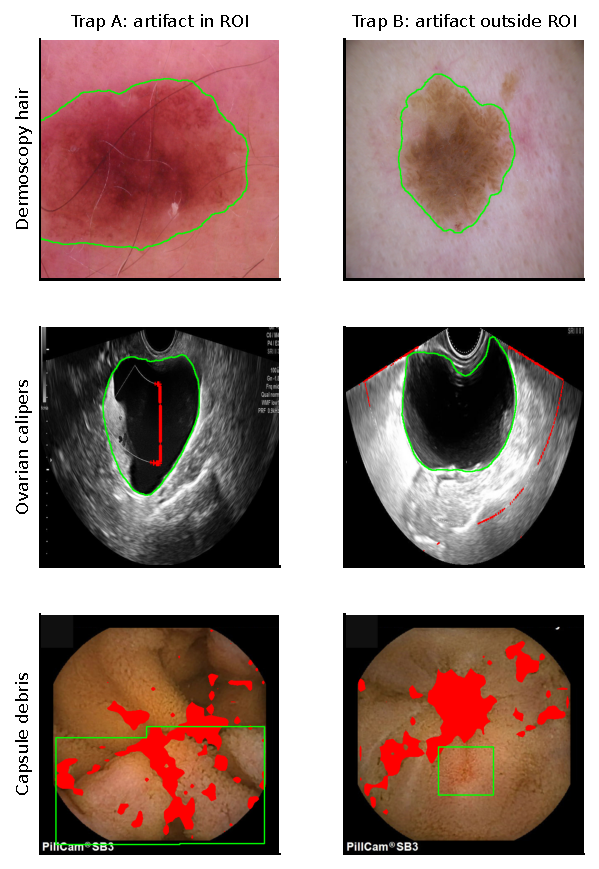
\includegraphics[width=0.62\linewidth]{figures/real_examples.pdf}
\caption{Real artifacts inside (Trap~A) and outside (Trap~B) the ROI. \textcolor{roigreen}{Green}: ROI;
\textcolor{artred}{red}: automatic artifact mask. Dermoscopy is shown with the lesion outline only, because the
published hair masks carry no licence that allows redistribution (overlays are kept locally). Thyroid images are not
shown (data licence not stated). Automatic overlap of the shown images: dermoscopy \sThreeExRisichairinroi{} and
\sThreeExRisichairoutroi; ovary \sThreeExRovarycalipersinroi{} and \sThreeExRovarycalipersoutroi; capsule
\sThreeExRcapsuledebrisinroi{} and \sThreeExRcapsuledebrisoutroi. ISIC CC BY-NC 4.0; MMOTU, SEE-AI CC BY 4.0.}
\label{fig:ex}\end{figure}
\paragraph{Mask validity} Table~\ref{tab:det}. Lesion masks are accurate (U-Net held-out Dice \sThreeUnetDice; against
HAM manual masks \sThreeUnetHam). The capsule debris probe reaches pixel accuracy \sThreeProbeAcc{} and IoU
\sThreeProbeIoU{} against expert masks. The thyroid caliper detector's detections lie on a real caliper in 38 of 40
audited images. The ovarian ``marker-free'' group is caliper-free but not overlay-free. The morphological hair detector
used for the pilot's counterfactual (E10) is poor (IoU \sThreeHairDetIoU), which is why all hair traps use the
published masks. Label noise in the artifact masks dilutes the constructed correlation and biases effects toward zero;
it cannot create a location difference by itself.
\begin{table}[H]\centering\scriptsize
\caption{Validity of the automatic masks that define artifact presence and location. Visual audits: \texttt{docs/ARTIFACT\_MASK\_AUDIT.md} (by the analysis agent, not a clinician; Stage~6 reports the blinded image audit prepared for a clinician).}\label{tab:det}
\begin{tabular}{p{3.0cm}p{3.0cm}p{3.8cm}p{4.6cm}}\toprule
Mask & Source & Check & Result \\\midrule
ISIC 2019 lesion masks (BCN, MSK) & U-Net trained on ISIC 2018 Task 1 & held-out Dice (mean) / Dice vs HAM manual masks & 0.886 / 0.895 \\
Hair (DullRazor-type detector, E10) & morphological & IoU / precision / recall vs Mendeley masks & 0.222 / 0.316 / 0.472 \\
Capsule debris masks & patch-token probe (2,160 expert-masked frames) & held-out pixel accuracy / IoU & 0.922 / 0.625 \\
Thyroid (TN3K), detected (A1) & visual audit, 40 images & detection lies on a real caliper / measurement mark & 38/40 (95 \%); 2 border false positives; 1 dotted zoom box (overlay) \\
Thyroid, marker-free (A0) & visual audit, 40 images & no visible caliper & 38–39/40 (95–97 \%); depth-scale ticks present in all images (not label-related) \\
Ovary (MMOTU), detected (A1) & visual audit, 40 images & an on-screen overlay is present & 40/40; caliper specifically 31/40 (others: dotted zoom arcs, focus markers, thumbnail inset) \\
Ovary, marker-free (A0) & visual audit, 40 images & no visible caliper & 37/40 (92 \%) \\
Ovary, marker-free (A0) & visual audit, 40 images & no overlay of any kind (arrows, boxes) & $\sim$29/40 (72 \%); text labels common \\
\bottomrule\end{tabular}
\end{table}


\subsection{The crossover with real artifacts}
Table~\ref{tab:traps} and Figure~\ref{fig:forest}. With DINOv2, masking is worse for in-ROI artifacts in every cohort:
\begin{itemize}[leftmargin=*]\itemsep1pt
\item \textbf{Dermoscopy hair.} Masking \emph{harms} when the hair lies on the lesion (\sThreeAisicDINOvTwo) and
helps when it lies outside (\sThreeBisicDINOvTwo); crossover \sThreeXisicDINOvTwo. After masking, the Trap~A model still
separates the correlated test (\sThreeMaskCorrAisicDINOvTwo) far better than the reversed one
(\sThreeMaskRevAisicDINOvTwo): the retained hair is used. The harm comes mainly from BCN images (\sThreeSrcBCN;
HAM \sThreeSrcHAM; Table~\ref{tab:src}; MSK is not reported separately).
\item \textbf{Thyroid calipers.} Masking helps in both traps but much more when the calipers lie outside the nodule
(\sThreeBthyroidDINOvTwo{} versus \sThreeAthyroidDINOvTwo; crossover \sThreeXthyroidDINOvTwo); with MedSigLIP the
crossover is \sThreeXthyroidMedSigLIP.
\item \textbf{Ovarian calipers.} Crossover \sThreeXovaryDINOvTwo{} (Trap~A \sThreeAovaryDINOvTwo, Trap~B
\sThreeBovaryDINOvTwo).
\item \textbf{Capsule debris.} The largest crossover (\sThreeXcapsuleDINOvTwo; MedSigLIP \sThreeXcapsuleMedSigLIP):
masking recovers almost all of the reversed-test loss when the debris lies outside the lesion box and little when it
lies on it.
\end{itemize}
The law in its real-artifact form is therefore a \emph{crossover}, and whether masking actually harms in Trap~A
depends on the cohort (it does for dermoscopy hair; for calipers and debris it helps less).
\begin{table}[H]\centering\scriptsize
\caption{Real-artifact traps: change in reversed-test AUROC from ROI masking, per trap, and the crossover (5 seeds $\times$ 5 grouped folds; crossed 95\% CIs).}\label{tab:traps}
\resizebox{\linewidth}{!}{\begin{tabular}{lccccc}\toprule
Cohort & Encoder & ERM reversed AUROC A / B & mask $-$ ERM, Trap A (in ROI) & mask $-$ ERM, Trap B (outside) & Crossover B $-$ A \\\midrule
Dermoscopy hair & DINOv2 & 0.510 / 0.510 & $-0.049$ [$-0.083, -0.018$] & $+0.098$ [$+0.060, +0.136$] & $+0.147$ [$+0.111, +0.185$] \\
Dermoscopy hair & DermLIP & 0.665 / 0.735 & $-0.104$ [$-0.143, -0.067$] & $-0.090$ [$-0.135, -0.046$] & $+0.014$ [$-0.037, +0.063$] \\
Thyroid calipers & DINOv2 & 0.289 / 0.405 & $+0.109$ [$+0.085, +0.133$] & $+0.348$ [$+0.307, +0.388$] & $+0.239$ [$+0.196, +0.280$] \\
Thyroid calipers & MedSigLIP & 0.289 / 0.481 & $+0.053$ [$+0.032, +0.073$] & $+0.248$ [$+0.200, +0.293$] & $+0.195$ [$+0.153, +0.238$] \\
Ovarian calipers & DINOv2 & 0.413 / 0.423 & $+0.132$ [$+0.072, +0.196$] & $+0.302$ [$+0.225, +0.378$] & $+0.170$ [$+0.087, +0.252$] \\
Capsule debris & DINOv2 & 0.581 / 0.429 & $+0.084$ [$+0.055, +0.112$] & $+0.461$ [$+0.415, +0.506$] & $+0.377$ [$+0.327, +0.426$] \\
Capsule debris & MedSigLIP & 0.570 / 0.464 & $+0.117$ [$+0.088, +0.147$] & $+0.452$ [$+0.407, +0.495$] & $+0.335$ [$+0.286, +0.383$] \\
\bottomrule\end{tabular}}
\end{table}

\begin{figure}[H]\centering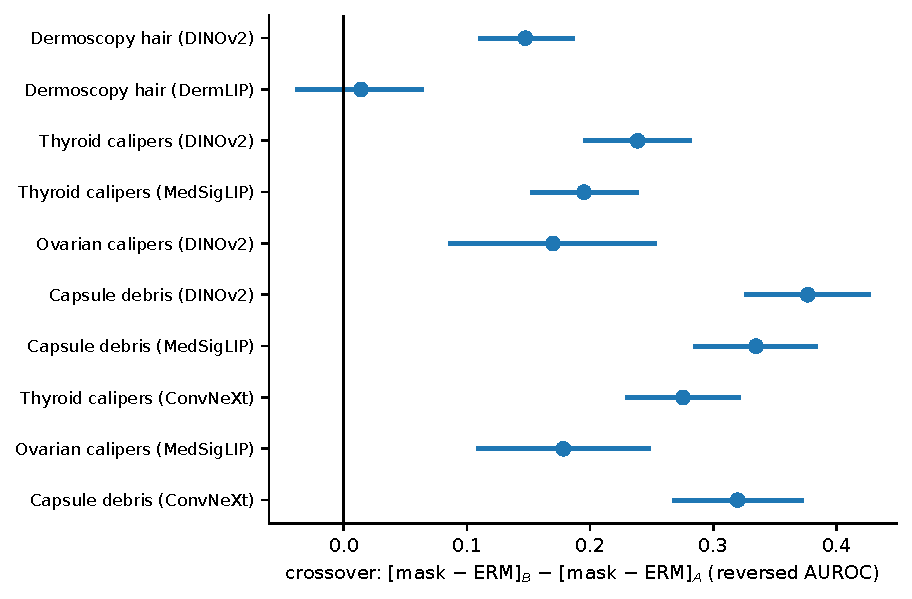
\includegraphics[width=0.78\linewidth]{figures/crossover_forest.pdf}
\caption{Crossover with real artifacts, per cohort and encoder (crossed 95\% CIs).}\label{fig:forest}\end{figure}
\begin{table}[H]\centering\small
\caption{Dermoscopy hair, Trap A, by image source (DINOv2).}\label{tab:src}
\begin{tabular}{lc}\toprule
Source & mask $-$ ERM, Trap A \\\midrule
HAM & $-0.011$ [$-0.064, +0.043$] \\
BCN & $-0.067$ [$-0.110, -0.025$] \\
\bottomrule\end{tabular}
\end{table}


\paragraph{Hair area relative to the lesion} In Trap~A the in-lesion hair covers a median \sThreeHairRatioMedian{} of
the lesion's area --- similar to the synthetic ruler of Stage~2. Split into tertiles of that ratio, masking harms in
every tertile (Table~\ref{tab:ratio}); unlike the synthetic sweep, no gradient across tertiles is visible, and the
intervals overlap.
\begin{table}[H]\centering\small
\caption{Dermoscopy hair, Trap A, by the ratio of in-lesion hair area to lesion area.}\label{tab:ratio}
\begin{tabular}{lcc}\toprule
Hair/lesion area tertile & Median ratio & mask $-$ ERM, Trap A \\\midrule
tertile 1 & 0.006 & $-0.057$ [$-0.095, -0.022$] \\
tertile 2 & 0.033 & $-0.046$ [$-0.082, -0.013$] \\
tertile 3 & 0.113 & $-0.037$ [$-0.071, -0.005$] \\
\bottomrule\end{tabular}
\end{table}


\subsection{The exception among encoders: DermLIP}
With DermLIP masking harms at \emph{both} hair locations (Trap~A \sThreeAisicDermLIP, Trap~B \sThreeBisicDermLIP) and
the crossover vanishes (\sThreeXisicDermLIP). DermLIP was trained on whole dermatology images and loses disease signal
when the background is removed, whatever the hair does. Stage~5 analyses this exception with the theory.

\subsection{The failed design: E12 overlap contrast}\label{sec:e12}
\begin{table}[H]\centering\small
\caption{E12 overlap-contrast design: hair inside the lesion ($A{=}1$, $r\ge0.5$) versus hair outside it ($A{=}0$, $r<0.1$), no artifact-free group (DINOv2, 5 seeds $\times$ 5 folds).}\label{tab:e12}
\begin{tabular}{lc}\toprule
Arm & change vs ERM (reversed AUROC) \\\midrule
ROI masking & $-0.103$ [$-0.121, -0.085$] \\
group-balanced & $+0.160$ [$+0.144, +0.177$] \\
DFR & $+0.179$ [$+0.148, +0.211$] \\
\bottomrule\end{tabular}
\end{table}

The pilot reported E12 as null. The re-implementation finds masking clearly harmful (\sThreeEOneTwomask), while group
balancing (\sThreeEOneTwobalanced) and DFR (\sThreeEOneTwodfr) help. As argued above, this is what the design
predicts whatever the location effect, because the label proxy \emph{is} location. The design was abandoned in favour of
the two-trap design with a shared artifact-free group; the pilot's null result is not supported.

\subsection{Chest radiography: the boundary}
In NIH radiographs linked to RANZCR-CLiP device annotations, Trap~A contains central venous catheters inside the lungs
and Trap~B endotracheal tubes outside them. Lung masking helped for both device types in all four registered findings
(Table~\ref{tab:cxr}); the registered claim that masking harms (or helps less) for the in-lung catheter was not
supported. The registration itself notes a confound: the catheter-free group carries many more out-of-lung tubes, which
masking removes. Together with the synthetic-tube sweep of Stage~2, where RAD-DINO ignored out-of-lung tubes, chest
radiography is the boundary of the law. The intervals of these runs were produced with the old estimator and cannot be
regenerated (the per-image predictions were not saved and the RANZCR data are not on this machine); they are withdrawn
and only point estimates are shown.
\begin{table}[H]\centering\small
\caption{Chest radiographs with real devices (NIH ChestX-ray14 linked to RANZCR-CLiP; RAD-DINO): Trap A = central venous catheter inside the lungs, Trap B = endotracheal tube outside them. Point estimates only, \textbf{not re-estimated} with the corrected bootstrap (per-image predictions were not saved; the old intervals are withdrawn).}\label{tab:cxr}
\begin{tabular}{lccc}\toprule
Finding (NIH, RANZCR-CLiP devices) & mask $-$ ERM, Trap A & Trap B & Crossover \\\midrule
Atelectasis & $+0.045$ & $+0.105$ & $+0.060$ \\
Consolidation & $+0.070$ & $+0.068$ & $-0.002$ \\
Effusion & $+0.104$ & $+0.100$ & $-0.004$ \\
Infiltration & $+0.094$ & $+0.063$ & $-0.032$ \\
\bottomrule\end{tabular}
\end{table}


\subsection{The 16-test primary family}
Table~\ref{tab:primary}. After Holm correction over all 16 tests, \sThreeNPrimaryOK{} of \sThreeNPrimary{} are
supported; all \sThreeNPOneOK{} location-crossover tests (P1) are supported. P2--P4 test remedies and are discussed in
Stage~6. Compared with the old estimator, one test lost support (P3, ovary: Holm $p$ \sThreePHolmPThreeOvary).
\begin{table}[H]\centering\small
\caption{The four pre-specified location tests (P1: crossover $>0$), crossed bootstrap, two-sided bootstrap $p$ (floored at $10^{-4}$), Holm-adjusted over the four cohorts.}\label{tab:primary}
\begin{tabular}{lcccc}\toprule
Cohort (DINOv2) & Crossover [95\% CI] & $p$ & $p$ (Holm, 4) & Supported \\\midrule
ISIC hair (DINOv2) & $+0.147$ [$+0.111, +0.185$] & 0.0001 & 0.0004 & \ok \\
Thyroid (DINOv2) & $+0.239$ [$+0.196, +0.280$] & 0.0001 & 0.0004 & \ok \\
Capsule (DINOv2) & $+0.377$ [$+0.327, +0.426$] & 0.0001 & 0.0004 & \ok \\
Ovary (DINOv2) & $+0.170$ [$+0.087, +0.252$] & 0.0001 & 0.0004 & \ok \\
\bottomrule\end{tabular}
\end{table}


\section{What failed or changed}
\begin{itemize}[leftmargin=*]\itemsep1pt
\item \textbf{E12 (pilot null) is not supported} and the design was abandoned for a structural reason.
\item \textbf{Chest-radiograph device traps}: the registered in-ROI harm was not supported (0 of 4 findings); their
old intervals are withdrawn because they could not be regenerated.
\item \textbf{DermLIP has no hair crossover}; the claim ``the crossover holds for every encoder'' is withdrawn.
\item \textbf{Primary family}: one test lost support with the corrected bootstrap (P3, ovary); \sThreeNPrimaryOK{} of
\sThreeNPrimary{} remain.
\item \textbf{The source strata of the hair trap} show that the Trap~A harm is carried by BCN images.
\item \textbf{The artifact masks were audited by the analysis agent, not by a clinician}; the blinded clinician audit
is prepared (Stage~6) but not yet done.
\end{itemize}

\section{Conclusion}
\textbf{Supported.} With real artifacts, masking is less useful when the artifact lies inside the ROI: the crossover is
positive in all four cohorts with DINOv2 and in both cohorts tested with MedSigLIP, and all four pre-specified crossover
tests survive Holm correction over 16. \textbf{Qualified.} Only for dermoscopy hair does masking actually harm in the
in-ROI trap; for calipers and debris it helps less. \textbf{Not supported.} A crossover with the dermatology encoder
DermLIP; an in-ROI penalty for real chest-radiograph devices; the pilot's null E12 result.

\section{Questions for the supervisor}
\begin{enumerate}\itemsep1pt
\item Is it acceptable that the artifact masks were validated by visual audit of the analysis agent until the
clinician audit (Stage~6) is done, or must the clinician audit precede submission?
\item The 16-test family was grouped after the individual results. Should the thesis present it as a post hoc
multiplicity safeguard (as here) or drop it in favour of per-cohort registration only?
\item Should chest radiography stay in the paper as a boundary case with point estimates only, or be moved to the
supplement until the device runs can be regenerated?
\end{enumerate}

\section{Next stage}
Real artifacts are not placed at random: the images whose hair lies on the lesion differ from those whose hair lies
beside it. Stage~4 asks whether the crossover survives when those differences are removed --- by matching on measured
covariates, by regression adjustment on the matched sample, and by moving the \emph{same} real artifact instance
inside and outside the ROI of the \emph{same} image --- and it reports the paste-edge control and every claim the
bootstrap correction changed.

\bibliographystyle{plainnat}
\bibliography{../common/references}
\end{document}
